\documentclass[11pt,a4paper]{article}
\usepackage[utf8]{inputenc}
\usepackage{amsmath,amsfonts,amssymb}
\usepackage{graphicx}
\usepackage{geometry}
\geometry{top=0.6in,bottom=0.6in,left=0.7in,right=0.7in}
\usepackage{booktabs}
\usepackage{hyperref}
\usepackage{float}
\usepackage{xcolor}

\definecolor{darkbg}{HTML}{0d121f}
\definecolor{lighttext}{HTML}{e2e8f0}
\definecolor{primary}{HTML}{8b5cf6}
\definecolor{secondary}{HTML}{0dd5c5}
\definecolor{accent}{HTML}{10b981}

\pagecolor{darkbg}
\color{lighttext}

\hypersetup{
    colorlinks=true,
    linkcolor=secondary,
    urlcolor=secondary,
    citecolor=accent
}

\title{\textbf{EE3621: Digital Signal Processing} \\ \Large Student Lecture Notes — Lecture 22 \\ \large Design of FIR Filters Using the Windowing Method}
\author{III B.Tech EEE — Core Exam Preparation Guide}
\date{}

\begin{document}

\maketitle

\noindent\rule{\textwidth}{0.5pt}

\section{Core Concept \& Principle of Windowing}

\subsection{The Truncation Problem \& Ideal Impulse Response Derivation}
An ideal brick-wall lowpass filter with cutoff frequency $\omega_c$ has the desired frequency response:
\begin{equation}
H_d(e^{j\omega}) = \begin{cases} 1, & |\omega| \le \omega_c \\ 0, & \omega_c < |\omega| \le \pi \end{cases}
\end{equation}
The continuous impulse response $h_d[n]$ is obtained via the **Inverse DTFT**:
\begin{align}
h_{d,\text{LP}}[n] &= \frac{1}{2\pi} \int_{-\pi}^{\pi} H_d(e^{j\omega}) e^{j\omega n} d\omega = \frac{1}{2\pi} \int_{-\omega_c}^{\omega_c} 1 \cdot e^{j\omega n} d\omega \nonumber \\
&= \frac{1}{2\pi} \left[ \frac{e^{j\omega n}}{jn} \right]_{-\omega_c}^{\omega_c} = \frac{e^{j\omega_c n} - e^{-j\omega_c n}}{2\pi j n}
\end{align}
Applying Euler's sine formula $e^{j\theta} - e^{-j\theta} = 2j\sin\theta$:
\begin{equation}
h_{d,\text{LP}}[n] = \frac{2j\sin(\omega_c n)}{2\pi j n} = \mathbf{\frac{\sin(\omega_c n)}{\pi n}}, \quad -\infty < n < \infty
\end{equation}
At $n = 0$, applying L'Hôpital's rule: $h_{d,\text{LP}}[0] = \lim_{n \to 0} \frac{\sin(\omega_c n)}{\pi n} = \mathbf{\frac{\omega_c}{\pi}}$.
This impulse response is doubly unphysical: it has **infinite duration (IIR)** and is **non-causal** (extends to $-\infty$).

To realize a physical causal FIR filter of length $N$, we:
\begin{enumerate}
    \item Shift the center of symmetry to $\tau = \alpha = \frac{N-1}{2}$ to ensure causality and linear phase.
    \item Multiply $h_d[n]$ pointwise by a finite-duration window sequence $w[n]$ ($0 \le n \le N-1$):
    \begin{equation}
    \mathbf{h[n] = h_d[n] \cdot w[n]}, \quad 0 \le n \le N-1
    \end{equation}
\end{enumerate}

\subsection{Frequency-Domain Convolution \& Gibbs Phenomenon}
By the DTFT modulation property, time-domain multiplication corresponds to periodic convolution in frequency:
\begin{equation}
H(e^{j\omega}) = \frac{1}{2\pi} H_d(e^{j\omega}) \circledast W(e^{j\omega}) = \frac{1}{2\pi} \int_{-\pi}^{\pi} H_d(e^{j\theta}) W(e^{j(\omega - \theta)}) d\theta
\end{equation}
\begin{itemize}
    \item \textbf{Mainlobe Width of $W(e^{j\omega})$:} Spreads out the ideal vertical transition into a gradual transition band $\Delta\omega$.
    \item \textbf{Sidelobes of $W(e^{j\omega})$:} Cause oscillations (ringing) in the passband and stopband.
    \item \textbf{Gibbs Phenomenon:} Abrupt rectangular truncation results in a fixed $8.95\%$ overshoot ($\approx -21$ dB peak sidelobe) near the discontinuity, which \textbf{cannot be reduced by increasing $N$}. Smoother, tapered windows are necessary to suppress sidelobes.
\end{itemize}

\newpage

\section{Master Window Summary Table (Formulas \& Specs)}

\begin{table}[H]
\centering
\caption{Characteristics of Standard FIR Filter Window Functions}
\label{tab:windows}
\vspace{2mm}
\resizebox{\textwidth}{!}{
\begin{tabular}{lcccc}
\toprule
\textbf{Window Name} & \textbf{Time-Domain Equation $w[n]$ ($0 \le n \le N-1$)} & \textbf{Transition Width $\Delta\omega$} & \textbf{Peak Sidelobe} & \textbf{Min. Attenuation $A_s$} \\
\midrule
\textbf{Rectangular} & $w[n] = 1$ & $\frac{4\pi}{N}$ (or $\frac{1.8\pi}{N}$) & $-13$ dB & $21$ dB \\
\textbf{Bartlett (Triangular)} & $w[n] = 1 - \frac{2|n - (N-1)/2|}{N-1}$ & $\frac{8\pi}{N}$ (or $\frac{6.1\pi}{N}$) & $-27$ dB & $25$ dB \\
\textbf{Hann (Hanning)} & $w[n] = 0.5 - 0.5\cos\left(\frac{2\pi n}{N-1}\right)$ & $\frac{8\pi}{N}$ (or $\frac{6.2\pi}{N}$) & $-32$ dB & $44$ dB \\
\textbf{Hamming} & $w[n] = 0.54 - 0.46\cos\left(\frac{2\pi n}{N-1}\right)$ & $\frac{8\pi}{N}$ (or $\frac{6.6\pi}{N}$) & $-43$ dB & $\mathbf{53 \text{ dB}}$ \\
\textbf{Blackman} & $w[n] = 0.42 - 0.5\cos\left(\frac{2\pi n}{N-1}\right) + 0.08\cos\left(\frac{4\pi n}{N-1}\right)$ & $\frac{12\pi}{N}$ (or $\frac{11\pi}{N}$) & $-58$ dB & $\mathbf{74 \text{ dB}}$ \\
\bottomrule
\end{tabular}
}
\end{table}

\begin{figure}[H]
\centering
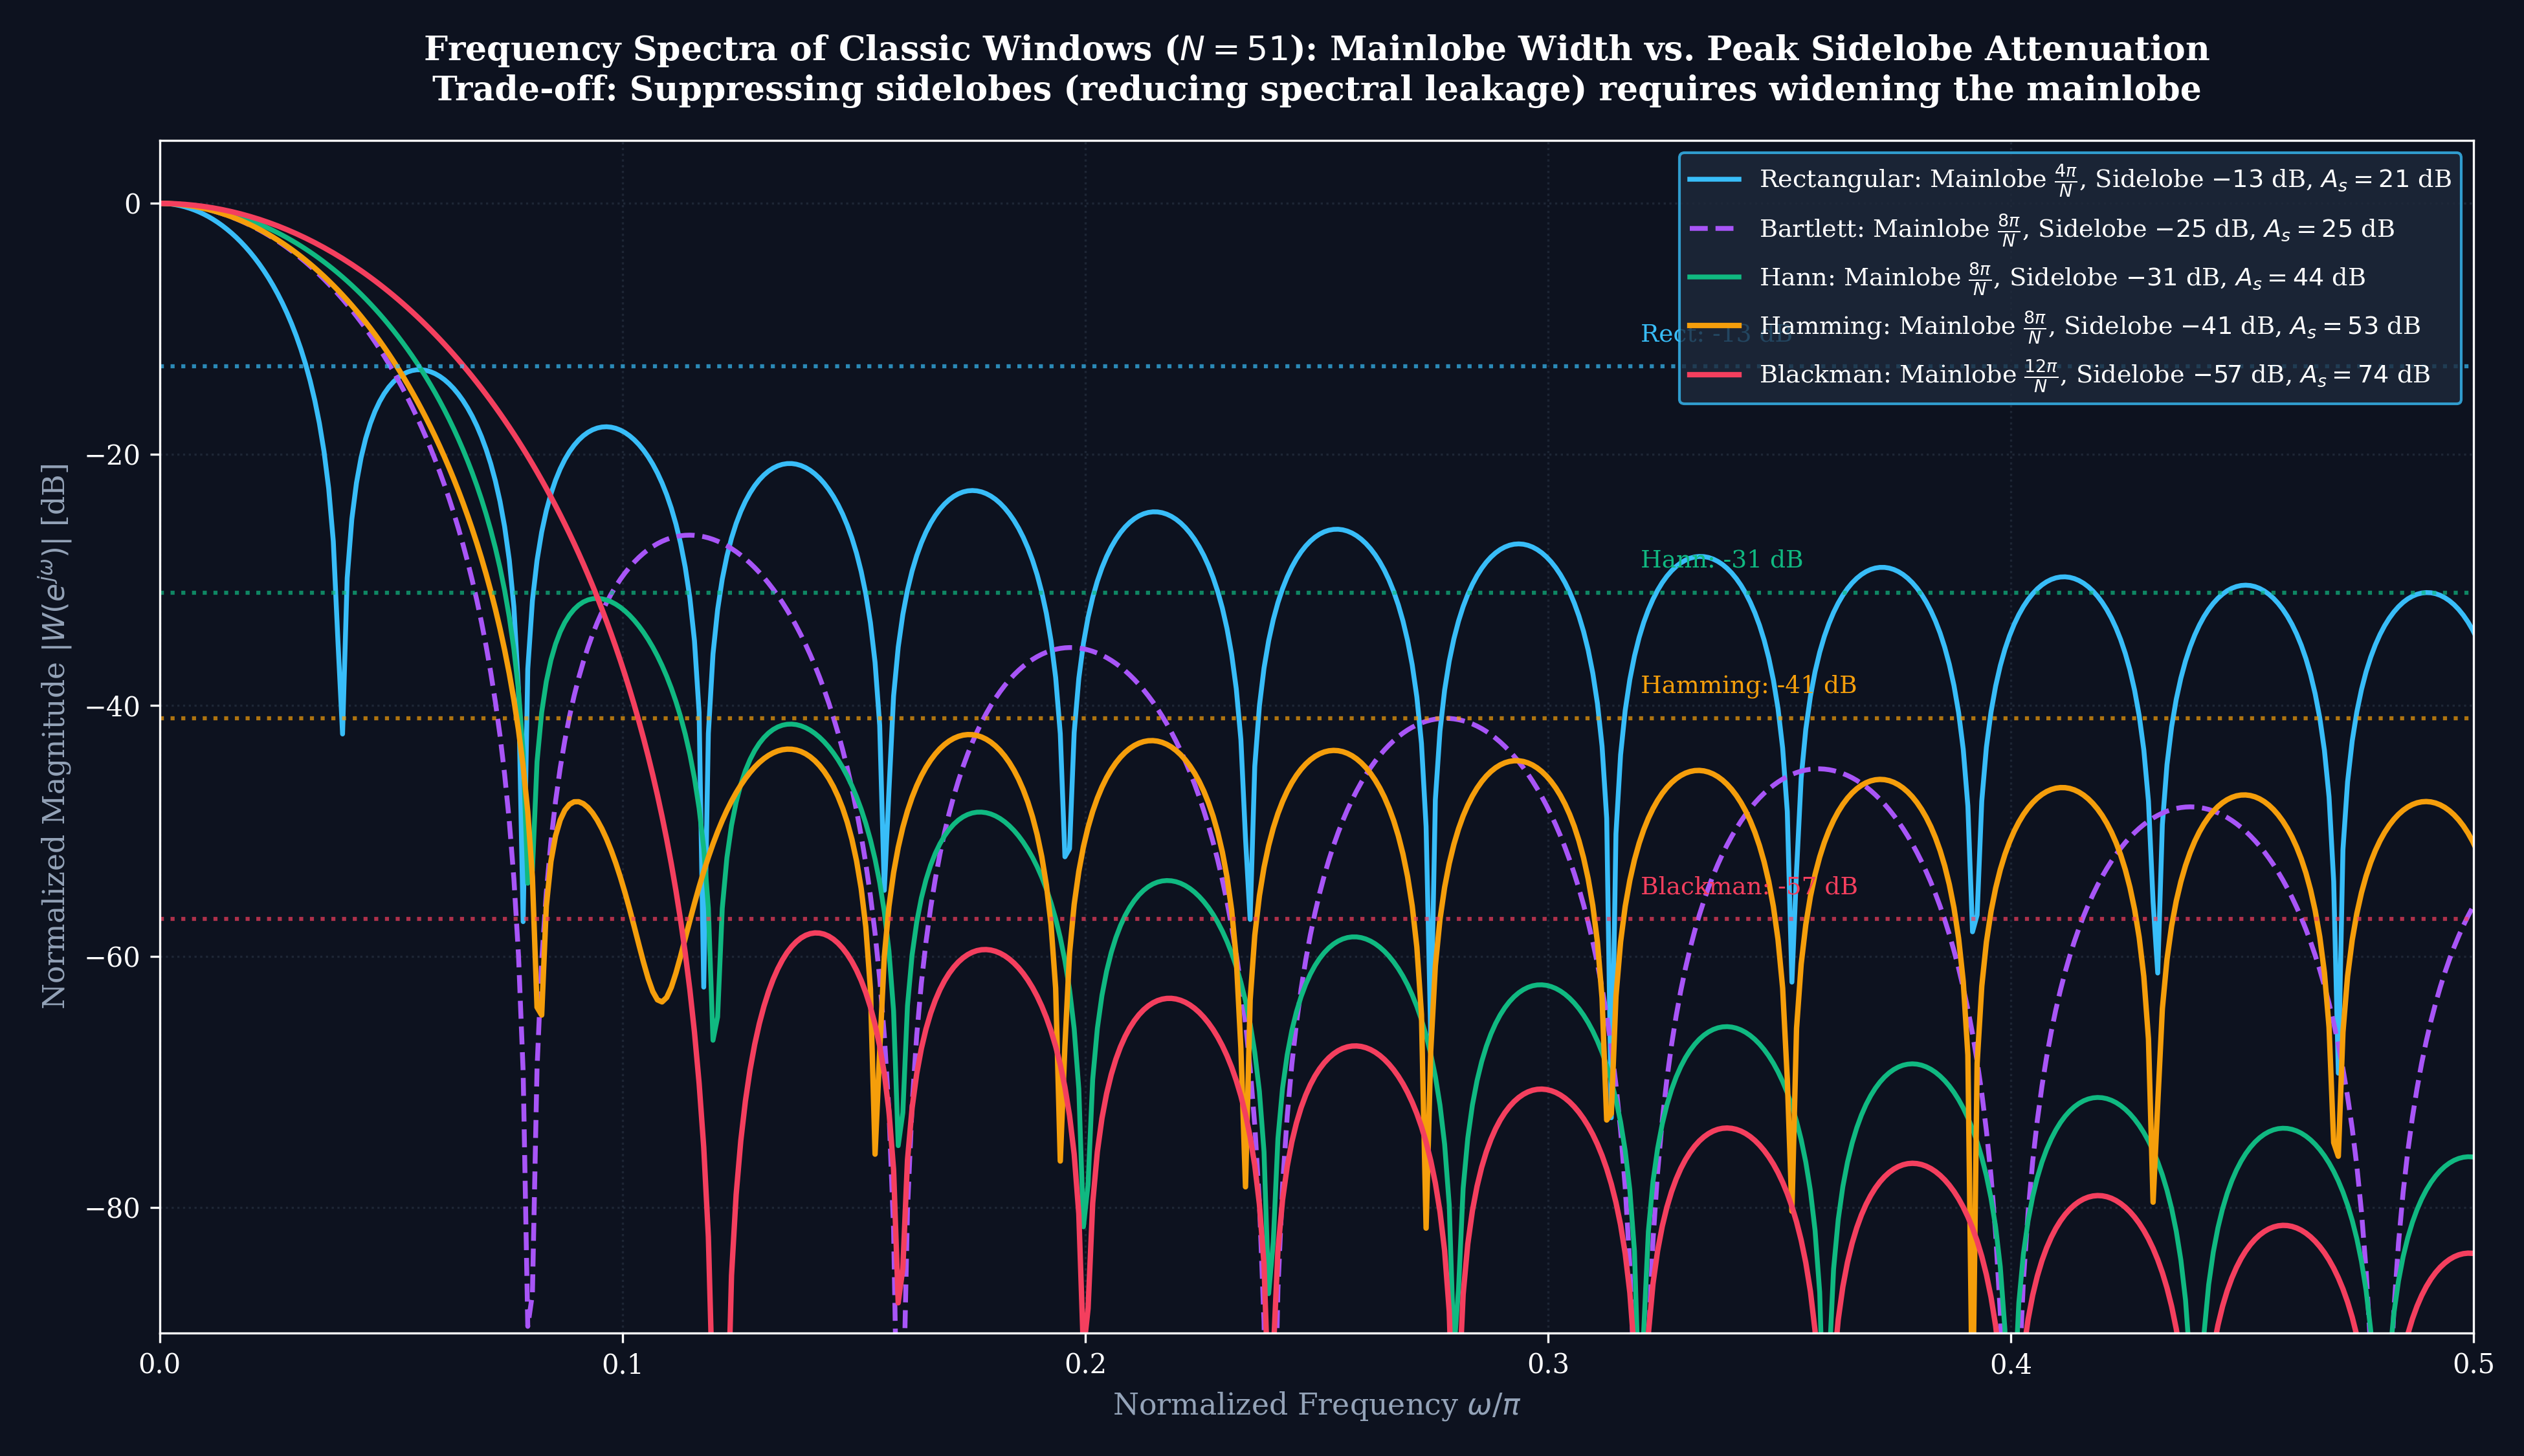
\includegraphics[width=0.82\textwidth]{images/fir_classic_windows_freq.png}
\caption{Normalized frequency magnitude spectra of classic window functions ($N = 51$). Note the fundamental trade-off: narrower mainlobe (faster transition roll-off) vs. lower sidelobes (higher stopband rejection).}
\label{fig:window_freq}
\end{figure}

\subsubsection*{Key Engineering Trade-offs \& Exam Rules:}
\begin{enumerate}
    \item \textbf{Mainlobe Width vs. Sidelobe Attenuation Trade-off:} As the window tapers more smoothly to zero at both ends (from Rectangular $\to$ Bartlett $\to$ Hann $\to$ Hamming $\to$ Blackman), the stopband attenuation improves dramatically from $21\text{ dB}$ to $74\text{ dB}$, but the mainlobe width expands from $4\pi/N$ to $12\pi/N$. A wider mainlobe requires a larger filter length $N$ to meet the same transition bandwidth $\Delta\omega$.
    \item \textbf{Why Hamming is the Universal Exam Default:} Hamming achieves $\mathbf{53\text{ dB}}$ stopband attenuation with the same mainlobe width ($\approx 8\pi/N$) as the Hann window ($44\text{ dB}$), because its nonzero pedestal ($0.08$) cancels the first sidelobe.
    \item \textbf{Why $N$ Cannot Reduce Sidelobes:} In fixed windows, increasing $N$ compresses the frequency axis (narrowing the mainlobe), but the \textbf{relative height of the sidelobes in dB remains constant}. Only choosing a different window type improves stopband attenuation $A_s$.
\end{enumerate}

\newpage

\section{Ideal Shifted Impulse Response Formulations}

To design a causal, linear-phase FIR filter of length $N$, the ideal frequency response incorporates a linear phase delay $\tau = \alpha = \frac{N-1}{2}$:
\begin{equation}
H_d(e^{j\omega}) = \begin{cases} 1 \cdot e^{-j\omega\tau}, & |\omega| \le \omega_c \\ 0, & \omega_c < |\omega| \le \pi \end{cases}
\end{equation}
Evaluating the Inverse DTFT with all intermediate integral steps:
\begin{align}
h_d[n] &= \frac{1}{2\pi} \int_{-\pi}^{\pi} H_d(e^{j\omega}) e^{j\omega n} d\omega = \frac{1}{2\pi} \int_{-\omega_c}^{\omega_c} e^{-j\omega\tau} e^{j\omega n} d\omega \nonumber \\
&= \frac{1}{2\pi} \int_{-\omega_c}^{\omega_c} e^{j\omega(n - \tau)} d\omega = \frac{1}{2\pi} \left[ \frac{e^{j\omega(n - \tau)}}{j(n - \tau)} \right]_{-\omega_c}^{\omega_c} \nonumber \\
&= \frac{e^{j\omega_c(n-\tau)} - e^{-j\omega_c(n-\tau)}}{2\pi j(n-\tau)} = \frac{2j\sin(\omega_c(n-\tau))}{2\pi j(n-\tau)} = \mathbf{\frac{\sin(\omega_c(n-\tau))}{\pi(n-\tau)}}, \quad n \ne \tau
\end{align}
At the center of symmetry $n = \tau$, applying L'H\^opital's rule:
\begin{equation}
h_d[\tau] = \lim_{n \to \tau} \frac{\sin(\omega_c(n-\tau))}{\pi(n-\tau)} = \lim_{n \to \tau} \frac{\omega_c\cos(\omega_c(n-\tau))}{\pi \cdot 1} = \mathbf{\frac{\omega_c}{\pi}}
\end{equation}

Highpass, bandpass, and bandstop filters follow directly from linear combinations of ideal lowpass filters:
\begin{itemize}
    \item \textbf{Highpass:} By spectral inversion, $H_{d,\text{HP}}(e^{j\omega}) = e^{-j\omega\tau} - H_{d,\text{LP}}(e^{j\omega}) \implies h_{d,\text{HP}}[n] = \delta[n-\tau] - h_{d,\text{LP}}[n]$.
    \item \textbf{Bandpass:} As difference of two lowpass filters, $h_{d,\text{BP}}[n] = h_{d,\text{LP2}}[n] - h_{d,\text{LP1}}[n]$.
    \item \textbf{Bandstop:} $h_{d,\text{BS}}[n] = \delta[n-\tau] - h_{d,\text{BP}}[n]$.
\end{itemize}

\begin{table}[H]
\centering
\caption{Closed-Form Formulas for Ideal Shifted Filters $h_d[n]$}
\label{tab:hd_formulas}
\vspace{2mm}
\begin{tabular}{lll}
\toprule
\textbf{Filter Type} & \textbf{For $n \ne \tau$} & \textbf{Center Tap $n = \tau$} \\
\midrule
\textbf{Lowpass (LPF)} & $h_d[n] = \frac{\sin(\omega_c(n-\tau))}{\pi(n-\tau)}$ & $h_d[\tau] = \frac{\omega_c}{\pi}$ \\
\textbf{Highpass (HPF)} & $h_d[n] = -\frac{\sin(\omega_c(n-\tau))}{\pi(n-\tau)}$ & $h_d[\tau] = 1 - \frac{\omega_c}{\pi}$ \\
\textbf{Bandpass (BPF)} & $h_d[n] = \frac{\sin(\omega_{c2}(n-\tau)) - \sin(\omega_{c1}(n-\tau))}{\pi(n-\tau)}$ & $h_d[\tau] = \frac{\omega_{c2} - \omega_{c1}}{\pi}$ \\
\textbf{Bandstop (BSF)} & $h_d[n] = \frac{\sin(\omega_{c1}(n-\tau)) - \sin(\omega_{c2}(n-\tau))}{\pi(n-\tau)}$ & $h_d[\tau] = 1 - \frac{\omega_{c2} - \omega_{c1}}{\pi}$ \\
\bottomrule
\end{tabular}
\end{table}

\subsection{Linear-Phase FIR Filter Constraints \& Symmetry Types}
To preserve exact linear phase without phase distortion, FIR impulse responses must satisfy symmetry:
\begin{itemize}
    \item \textbf{Type 1 (Symmetric, $N$ Odd):} Impulse response satisfies $h[n] = h[N-1-n]$ with integer delay $\tau = \frac{N-1}{2}$. The center sample is at an integer index $n = \tau$. Type 1 filters can realize \textbf{all four filter classes} (Lowpass, Highpass, Bandpass, and Bandstop).
    \item \textbf{Type 2 (Symmetric, $N$ Even):} Symmetrical about a half-integer $\tau = \frac{N-1}{2}$. This symmetry strictly forces a null at $\omega = \pi$: $H(e^{j\pi}) = 0$. Therefore, \textbf{an even-length symmetric filter can NEVER be used for Highpass or Bandstop filters} where transmission at $\omega = \pi$ is required!
    \item \textbf{Design Takeaway for Exams:} Always verify that $N$ is chosen \textbf{odd} for highpass or bandstop designs, guaranteeing full passband transmission at Nyquist ($\omega = \pi$).
\end{itemize}

\newpage

\section{FIR Filter Specifications \& 5-Step Window Design Procedure}

\subsection{Filter Tolerance Specifications \& Frequency Bands}
To design a physical FIR filter using the windowing method, the ideal brick-wall response must be approximated within acceptable engineering tolerance bands, as illustrated in Figure \ref{fig:filter_specs}:

\begin{figure}[H]
\centering
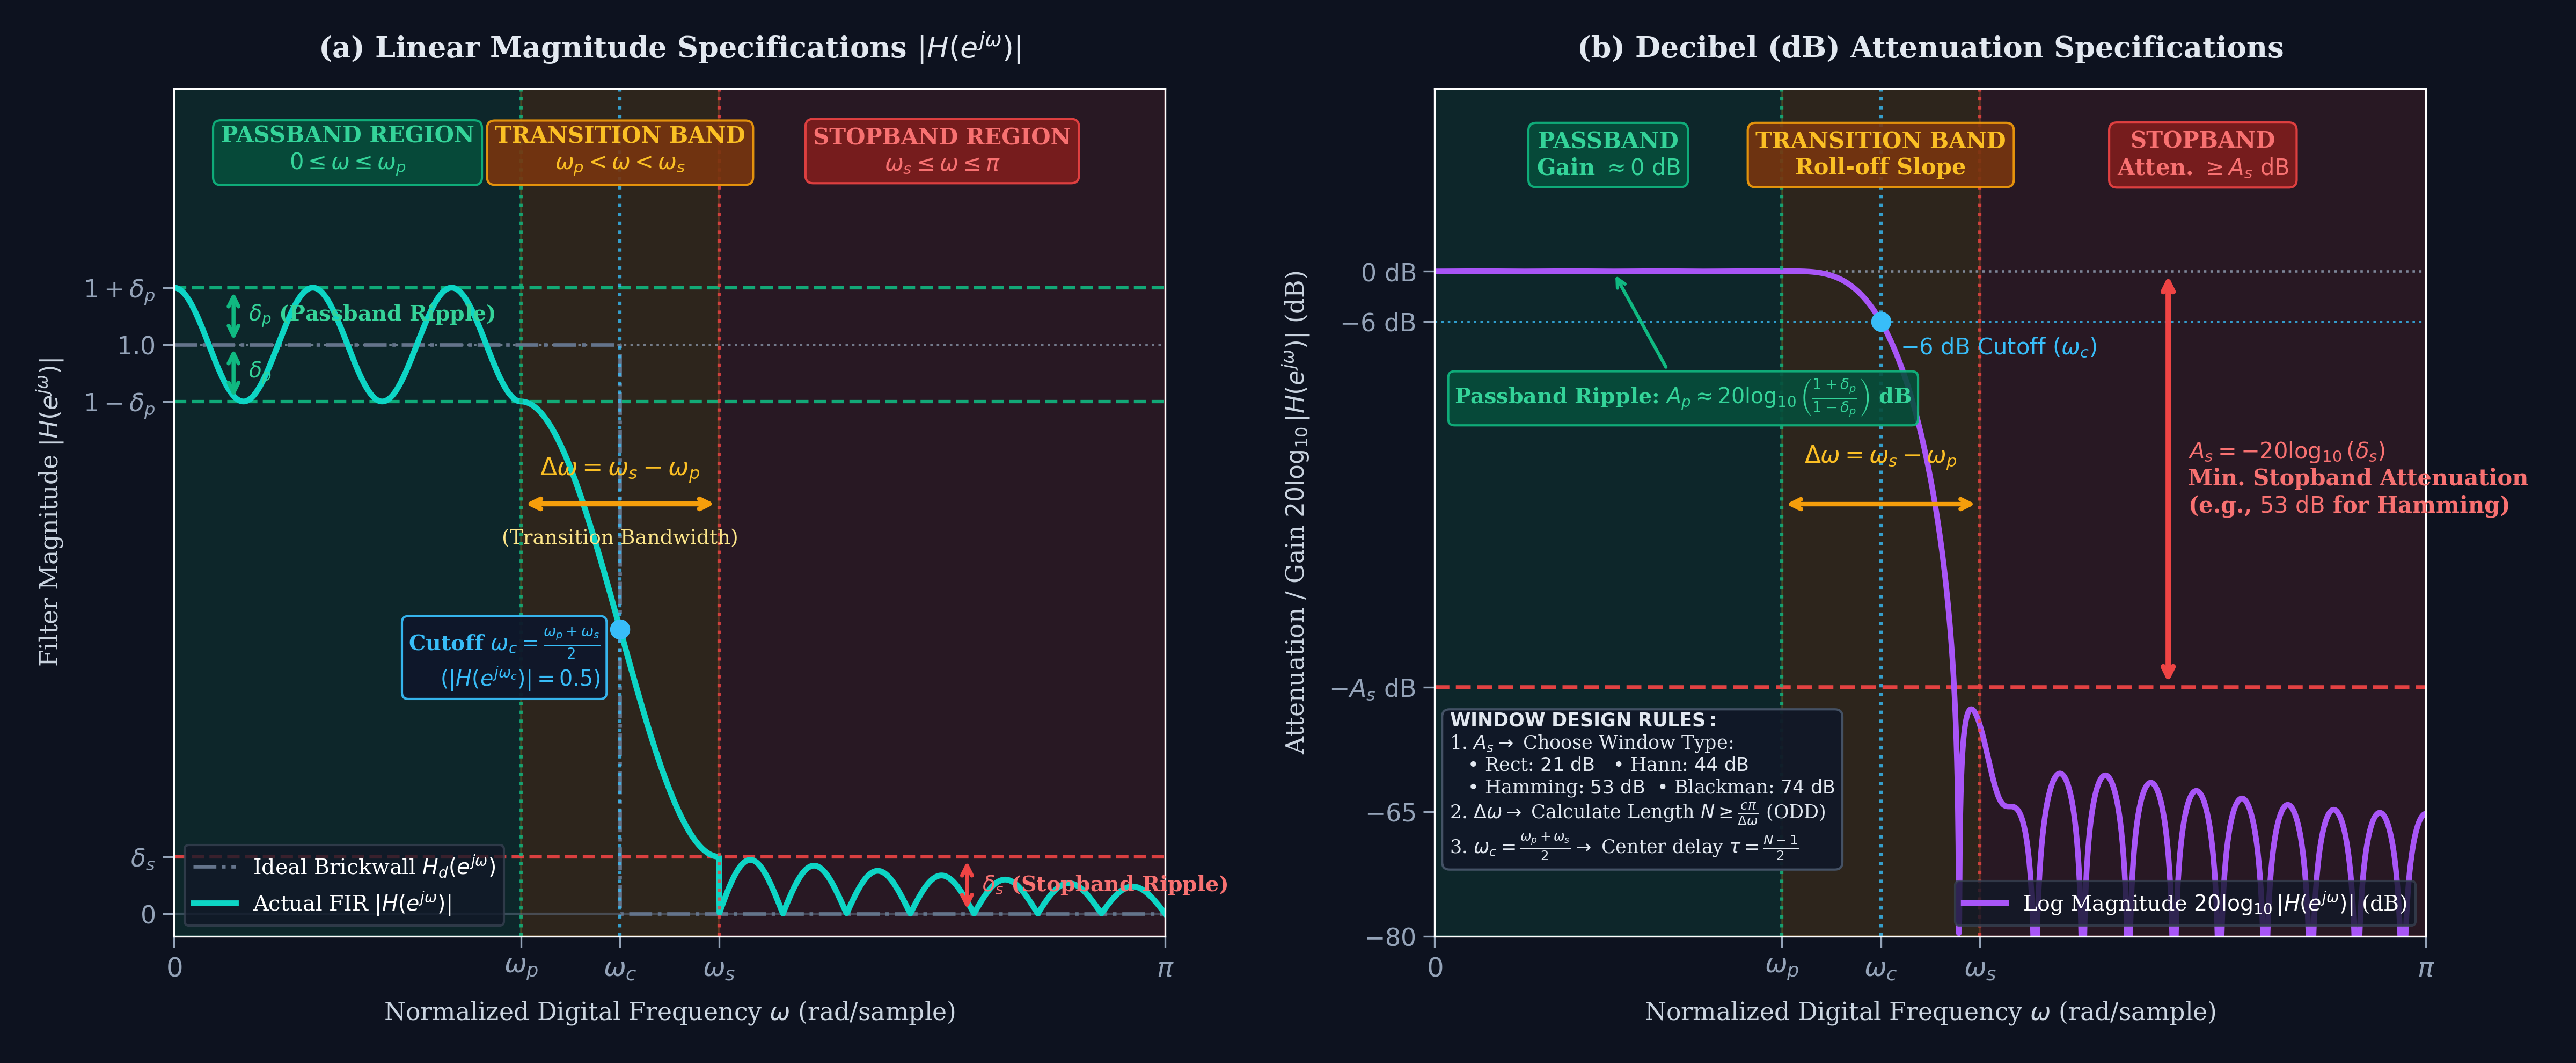
\includegraphics[width=0.80\textwidth]{images/fir_filter_specs_tolerance.png}
\caption{FIR Filter Tolerance Specifications and Parameter Mapping: (a) Linear magnitude $|H(e^{j\omega})|$ displaying passband ripple $\delta_p$, stopband ripple $\delta_s$, transition bandwidth $\Delta\omega = \omega_s - \omega_p$, and $-6$ dB cutoff frequency $\omega_c = (\omega_p + \omega_s)/2$; (b) Decibel attenuation showing minimum stopband attenuation $A_s = -20\log_{10}(\delta_s)$ dB and systematic window design mapping.}
\label{fig:filter_specs}
\end{figure}

\begin{itemize}
    \item \textbf{Passband ($0 \le \omega \le \omega_p$):} Band where desired frequencies pass. The magnitude stays bounded within $1 - \delta_p \le |H(e^{j\omega})| \le 1 + \delta_p$. Peak-to-peak ripple is $2\delta_p$, and passband ripple in decibels is $A_p \approx 20\log_{10}\frac{1+\delta_p}{1-\delta_p}$ dB.
    \item \textbf{Transition Band ($\omega_p < \omega < \omega_s$):} Finite roll-off band connecting passband and stopband. The \textbf{transition bandwidth} $\mathbf{\Delta\omega = \omega_s - \omega_p}$ is governed by the window mainlobe width ($\Delta\omega \approx \frac{c\pi}{N}$), which \textbf{dictates the minimum filter length $N$}.
    \item \textbf{Cutoff Frequency ($\omega_c$):} The ideal transition midpoint where gain drops to $0.5$ ($-6$ dB attenuation): $\mathbf{\omega_c = \frac{\omega_p + \omega_s}{2}}$.
    \item \textbf{Stopband ($\omega_s \le \omega \le \pi$):} Band where unwanted frequencies are suppressed: $|H(e^{j\omega})| \le \delta_s$. The \textbf{minimum stopband attenuation} $\mathbf{A_s = -20\log_{10}(\delta_s)\text{ dB}}$ is governed by the window peak sidelobe, which \textbf{dictates the choice of window type} (independent of $N$).
\end{itemize}

\subsection{The 5-Step Systematic Design Procedure}
\begin{enumerate}
    \item \textbf{Step 1 — Identify Stopband Attenuation $A_s$:} From $\delta_s$, calculate $A_s = -20\log_{10}(\delta_s)$ dB. Select the window from Table \ref{tab:windows} whose peak sidelobe attenuation meets or exceeds $A_s$.
    \item \textbf{Step 2 — Calculate Filter Length $N$:} From $\Delta\omega = \omega_s - \omega_p$, determine $N \ge \frac{c\pi}{\Delta\omega}$ from Table \ref{tab:windows}. Round up to the \textbf{next odd integer} to ensure Type 1 linear phase (integer delay $\tau = (N-1)/2$).
    \item \textbf{Step 3 — Determine Cutoff Frequency $\omega_c$:} Set $\omega_c = \frac{\omega_p + \omega_s}{2}$.
    \item \textbf{Step 4 — Formulate Shifted Ideal Impulse Response $h_d[n]$:} Evaluate $h_d[n]$ for $n = 0, 1, \dots, N-1$ using Table \ref{tab:hd_formulas} with delay $\tau = \frac{N-1}{2}$.
    \item \textbf{Step 5 — Apply Window Multiplication:} Compute final filter coefficients: $h[n] = h_d[n] \cdot w[n]$.
\end{enumerate}

\newpage

\section{Standard Solved Exam Example 1: Lowpass Filter Design}

\textbf{Problem:} Design a linear-phase FIR lowpass filter with cutoff frequency $\omega_c = 0.5\pi$ rad/sample and length $N = 7$ using a \textbf{Hamming window}. Determine impulse response $h[n]$, system function $H(z)$, and verify frequency response at $\omega = 0$ (DC) and $\omega = \pi$ (Nyquist).

\vspace{1mm}
\noindent\textbf{Solution:}

\noindent\textbf{Step 1: Symmetry Delay Parameter} \\
For length $N = 7$ (odd), the center of symmetry is $\tau = \alpha = \frac{N - 1}{2} = \frac{7 - 1}{2} = \mathbf{3}$ (integer delay $\implies$ Type 1 FIR).

\vspace{1mm}
\noindent\textbf{Step 2: Ideal Shifted Impulse Response Evaluation $h_d[n]$} \\
From Table \ref{tab:hd_formulas}, the shifted ideal LPF formula with $\omega_c = 0.5\pi$ is $h_d[n] = \frac{\sin(0.5\pi(n-3))}{\pi(n-3)}$ for $n \ne 3$, and center tap $h_d[3] = \frac{\omega_c}{\pi} = \frac{0.5\pi}{\pi} = \mathbf{0.5000}$. Evaluating taps:
\begin{align}
n = 2: &\; h_d[2] = \tfrac{\sin(0.5\pi(-1))}{-\pi} = \tfrac{-1}{-\pi} = \tfrac{1}{\pi} \approx \mathbf{0.3183} &
n = 1: &\; h_d[1] = \tfrac{\sin(-\pi)}{-2\pi} = \mathbf{0.0000} \nonumber \\
n = 0: &\; h_d[0] = \tfrac{\sin(-1.5\pi)}{-3\pi} = \tfrac{1}{-3\pi} = -\tfrac{1}{3\pi} \approx \mathbf{-0.1061}
\end{align}
By even symmetry about $\tau = 3$ ($h_d[3+k] = h_d[3-k]$):
$h_d[4] = h_d[2] = 0.3183$, $h_d[5] = h_d[1] = 0.0000$, and $h_d[6] = h_d[0] = -0.1061$.

\vspace{1mm}
\noindent\textbf{Step 3: Hamming Window Weights $w[n]$} \\
The formula for a length-$7$ Hamming window ($0 \le n \le 6$) is $w[n] = 0.54 - 0.46\cos\left(\frac{2\pi n}{6}\right) = 0.54 - 0.46\cos\left(\frac{\pi n}{3}\right)$:
\begin{align}
n = 3: &\; w[3] = 0.54 - 0.46(-1) = \mathbf{1.0000} & n = 2: &\; w[2] = 0.54 - 0.46(-0.5) = \mathbf{0.7700} \nonumber \\
n = 1: &\; w[1] = 0.54 - 0.46(0.5) = \mathbf{0.3100} & n = 0: &\; w[0] = 0.54 - 0.46(1) = \mathbf{0.0800}
\end{align}
By window symmetry: $w[4] = w[2] = 0.7700$, $w[5] = w[1] = 0.3100$, $w[6] = w[0] = 0.0800$.

\vspace{1mm}
\noindent\textbf{Step 4: Windowing Multiplication $h[n] = h_d[n] \cdot w[n]$} \\
Multiplying corresponding values tap-by-tap: \\
$h[3] = 0.50000 \times 1.0000 = \mathbf{0.5000}$, \quad
$h[2] = h[4] = 0.31831 \times 0.7700 = \mathbf{0.2451}$, \\
$h[1] = h[5] = 0.00000 \times 0.3100 = \mathbf{0.0000}$, \quad
$h[0] = h[6] = -0.10610 \times 0.0800 = \mathbf{-0.0085}$.
\begin{equation}
\mathbf{h[n] = \{-0.0085, \; 0.0000, \; 0.2451, \; \underset{\uparrow}{0.5000}, \; 0.2451, \; 0.0000, \; -0.0085\}}
\end{equation}

\noindent\textbf{Step 5: System Function $H(z)$ and Frequency Response Verification} \\
Transfer function: $H(z) = -0.0085 + 0.2451 z^{-2} + 0.5000 z^{-3} + 0.2451 z^{-4} - 0.0085 z^{-6}$. \\
Factoring linear phase delay $e^{-j 3\omega}$ on the unit circle $z = e^{j\omega}$:
\begin{align}
H(e^{j\omega}) &= e^{-j 3\omega} \left[ h[3] + 2h[2]\cos(\omega) + 2h[1]\cos(2\omega) + 2h[0]\cos(3\omega) \right] \nonumber \\
&= e^{-j 3\omega} \left[ 0.5000 + 2(0.2451)\cos(\omega) + 0 - 2(0.0085)\cos(3\omega) \right] \nonumber \\
&= e^{-j 3\omega} \left[ 0.5000 + 0.4902\cos(\omega) - 0.0170\cos(3\omega) \right]
\end{align}
\noindent\textbf{Critical Frequency Verification:}
\begin{itemize}
    \item \textbf{DC Gain ($\omega = 0$):} With $\cos(0) = 1$:
    $H(e^{j0}) = 0.5000 + 0.4902(1) - 0.0170(1) = \mathbf{0.9732} \approx 1.0$ (ideal passband transmission).
    \item \textbf{Nyquist Gain ($\omega = \pi$):} With $\cos(\pi) = \cos(3\pi) = -1$:
    $H(e^{j\pi}) = e^{-j 3\pi} [0.5000 - 0.4902 + 0.0170] = (-1) \cdot [0.0268] = \mathbf{-0.0268}$. \\
    Stopband attenuation at $\pi$: $|H(e^{j\pi})| = 0.0268 \implies 20\log_{10}(0.0268) \approx \mathbf{-31.44\text{ dB}}$, verifying strong lowpass attenuation with only 7 taps.
\end{itemize}

\newpage

\section{Solved Exam Example 2: Highpass Filter Design}

\textbf{Problem:} Design a 5-tap linear-phase FIR highpass filter with cutoff frequency $\omega_c = 0.5\pi$ rad/sample using a \textbf{Rectangular window}. Determine $h[n]$ and verify its frequency response at $\omega = 0$ and $\omega = \pi$.

\vspace{1mm}
\noindent\textbf{Solution:}

\noindent\textbf{Step 1: Symmetry Delay Parameter} \\
Filter length $N = 5 \implies \tau = \frac{5 - 1}{2} = \mathbf{2}$.

\vspace{1mm}
\noindent\textbf{Step 2: Ideal Shifted Highpass Impulse Response $h_d[n]$} \\
From Table \ref{tab:hd_formulas}, the shifted ideal highpass formula is:
\begin{equation}
h_d[n] = \begin{cases} 1 - \dfrac{\omega_c}{\pi} = 1 - \dfrac{0.5\pi}{\pi} = 0.5000, & n = \tau = 2 \\[6pt] -\dfrac{\sin(0.5\pi(n-2))}{\pi(n-2)}, & n \ne 2 \end{cases}
\end{equation}
Evaluating each tap explicitly:
\begin{align}
n = 2: &\; h_d[2] = 1 - 0.5 = \mathbf{0.5000} \nonumber \\
n = 1: &\; h_d[1] = -\frac{\sin(0.5\pi(-1))}{-\pi} = -\frac{-1}{-\pi} = -\frac{1}{\pi} \approx \mathbf{-0.3183} \nonumber \\
n = 0: &\; h_d[0] = -\frac{\sin(0.5\pi(-2))}{-2\pi} = -\frac{0}{-2\pi} = \mathbf{0.0000}
\end{align}
By even symmetry about $\tau = 2$: $h_d[3] = h_d[1] = -0.3183$ and $h_d[4] = h_d[0] = 0.0000$.

\vspace{1mm}
\noindent\textbf{Step 3: Rectangular Window \& Multiplication} \\
For a rectangular window, $w[n] = 1$ for $0 \le n \le 4$. Therefore $h[n] = h_d[n]$:
\begin{equation}
\mathbf{h[n] = \{0.0000, \; -0.3183, \; \underset{\uparrow}{0.5000}, \; -0.3183, \; 0.0000\}}
\end{equation}

\noindent\textbf{Step 4: Frequency Response Verification}
\begin{equation}
H(e^{j\omega}) = e^{-j 2\omega} [h[2] + 2h[1]\cos(\omega) + 2h[0]\cos(2\omega)] = e^{-j 2\omega} [0.5000 - 0.6366\cos(\omega)]
\end{equation}
\begin{itemize}
    \item \textbf{Stopband at DC ($\omega = 0$):} $H(e^{j0}) = 0.5000 - 0.6366(1) = \mathbf{-0.1366} \approx 0$ (attenuated).
    \item \textbf{Passband at Nyquist ($\omega = \pi$):} $H(e^{j\pi}) = e^{-j 2\pi}[0.5000 - 0.6366(-1)] = 1 \cdot [0.5000 + 0.6366] = \mathbf{1.1366} \approx 1$ (passed).
\end{itemize}

\noindent\rule{\textwidth}{0.5pt}

\section{Essential Exam Checklist \& Traps}
\begin{itemize}
    \item[$\square$] \textbf{Center Tap Formula:} For LPF, $h_d[\tau] = \omega_c/\pi$. Do NOT attempt $\frac{\sin(0)}{0}$ without taking the limit!
    \item[$\square$] \textbf{Highpass Inversion:} For HPF, $h_d[\tau] = 1 - \omega_c/\pi$. All other taps are the negative of the LPF taps.
    \item[$\square$] \textbf{Window Selection Rule:} If the specification requires $A_s = 50$ dB, a Hann window ($A_s = 44$ dB) is insufficient. You \textbf{must select Hamming} ($A_s = 53$ dB).
    \item[$\square$] \textbf{Argument in Window Cosine:} Remember the denominator is $N-1$, not $N$: $\cos\left(\frac{2\pi n}{N-1}\right)$.
\end{itemize}

\end{document}
